\chapter{Números/Relações (2º Bimestre)}

\section{Matrizes}

An $m$-by-$n$ matrix $A$ is a table with $m$ rows and $n$ columns, for
example
%%
    $$
    A = \begin{pmatrix}
       1 & -7.7 & 2 & \frac{1}{3} \\
       \frac{3}{2} & \sqrt{2} & 0 & -\pi^2 \\
       -2.5 & 0 & 7 & \sqrt[3]{40}
    \end{pmatrix}
    $$

The $m \times n$ elements of the matrix are called the coefficients of the
matrix. The integers $m,n$ are called the dimensions of the matrix or said to
characterize the size of the matrix. It is customary to use uppercase letters
to denote matrices (e.g. $A$) and to use lowercase letters for the coefficients
of the matrix (e.g. $a_{i,j}$ for the one at row $1 \leq i \leq n$ and column
$1 \leq j \leq m$).

We have special cases for the dimension of the matrix.
When $m = n$ the matrix is called a square matrix ;
when $n = 1$ it is called a column vector ; when $m = 1$ it is called a row
vector ; finally if $m = n = 1$ there is an obvious identification
$(\alpha) \leftrightarrow \alpha$ between the matrix with a single element and
the element itself.

We also have special cases according to the coefficients.
A matrix is upper triangular matrix if all the elements below the diagonal are
zero. A matrix is lower triangular matrix if all the elements above the diagonal
are zero. A matrix is diagonal if all the elements outside the diagonal are
zero. If $A$ is a square matrix of size $n$, then $A$ is symmetric iff
$a_{ij} = a_{ji}$ for $1 \leq i \leq j \leq n$ and antisymmetric iff
$a_{ij} = -a_{ji}$ for $1 \leq i \leq j \leq n$.

\subsection*{Exercício 1}

Indicate the dimensions of the following matrices, an expression of the
coefficients $a_{i,j}$ and whether they have special properties.

\begin{enumerate}
\item
    $$A=\begin{pmatrix}
       \frac{1}{2} & 0 & 0 \\
       0 & 1 & 0 \\
       0 & 0 & \frac{3}{2}
    \end{pmatrix}$$

\item
    $$B=\begin{pmatrix}
       1 & 1 & 1 & 1 & 1 \\
       0 & 1 & 1 & 1 & 1 \\
       0 & 0 & 1 & 1 & 1 \\
       0 & 0 & 0 & 1 & 1
    \end{pmatrix}$$

\item
    $$C=\begin{pmatrix}
       1 & 0 & 0 & 0 \\
       -1 & 2 & 0 & 0 \\
       1 & -1 & 3 & 0 \\
       -1 & 1 & -1 & 4 \\
    \end{pmatrix}$$

\item
    $$D=\begin{pmatrix}
       2 & 3 & 4 \\
       3 & 4 & 5 \\
       4 & 5 & 6 \\
       5 & 6 & 7 \\
    \end{pmatrix}$$

\item
  $$E=\begin{pmatrix}
       0 & 2 & 3 \\
       -2 & 0 & 3 \\
       -3 & -3 & 0
    \end{pmatrix}$$
\end{enumerate}

Given two matrices $A$ and $B$ with the same dimensions
$m,n$ we can define a new $m$-by-$n$ matrix $C$ like this:
$c_{i,j} = a_{i,j} + b_{i,j}$ for $1\leq i \leq m$ and
$1\leq j \leq n$. Concretely, we sum up the two coefficients of
$A$ and $B$ at a given position. We denote this matrix $C=A+B$ and
call it the sum of $A$ and $B$. If we consider this operation for
1-by-1 matrices, we see that this generalizes the sum of numbers.
As for numbers, it is easy to see that the addition is associative
and commutative: given three matrices $A,B,C$ of same dimensions we have
$(A+B)+C = A+(B+C)$ and $A+B = B+A$.
The $m$-by-$n$ zero-matrix is the matrix whose coefficients are all
zero and is denoted $0_{m,n}$ or
$0$ when size is clear from the context.
Again, it is easy check that for any other $m$-by-$n$ matrix $A$,
we have $0 + A = 0 + A = A$. Given an
$m$-by-$n$ matrix $A$, we denote $-A$ the $m$-by-$n$
matrix whose coefficients are $-a_{i,j}$ for $1\leq i \leq m$ and
$1\leq j \leq n$. Then $A + -A = -A + A = 0$.
Given two $m$-by-$n$ matrices $A,B$ we note $A - B = A + -B$ the
subtraction of the two matrices $A$ and $B$. Equivalently,
it is defined by the coefficients
$a_{i,j} - b_{i,j}$ for $1\leq i \leq m$ and $1\leq j \leq n$.

\subsection*{Exercício 2}

Perform the following operations, when they are well-defined.

\begin{enumerate}
\item The sum of $\begin{pmatrix}
  2 & 3 & 4 \\
  3 & 4 & 5 \\
  4 & 5 & 6 \\
\end{pmatrix}$ and $\begin{pmatrix}
  2 & 7 & 2 \\
  -1 & 3 & -1 \\
\end{pmatrix}$

\item $\begin{pmatrix}
  8 & 3 & 4 \\
  3 & 4 & 9 \\
\end{pmatrix} - \begin{pmatrix}
  2 & 7 & 2 \\
  -1 & 3 & -1 \\
\end{pmatrix}$

\item $\begin{pmatrix}
  8 & 3 \\
  3 & 4
\end{pmatrix} + \begin{pmatrix}
  11 & 0 \\
  2 & 4
\end{pmatrix} + \begin{pmatrix}
  0 & 2 \\
  0 & 1
\end{pmatrix}$

\item $-\begin{pmatrix}
  8 & 3 & 4 \\
  3 & 4 & 9 \\
  5 & 0 & 2 \\
  11 & 4 & 0
\end{pmatrix}$
\end{enumerate}

We consider a one $m$-by-$n$ matrix $A$ and one $n$-by-$p$ matrix $B$
(the number of
columns of $A$ is equal to the number of rows of $B$). We can define a new
$m$-by-$p$ matrix $C$ like this:
%%
      $$c_{i,j} = \sum_{k=1}^n a_{i,k} b_{k,j}$$
%%
for $1\leq i \leq m$ and $1\leq j \leq p$. We denote this matrix $C = A B$ and
call it the product of $A$ and $B$. Visually, the above formula is interpreted
by considering the $i$-th row of $A$ and the $j$-th column of $B$. By
assumption, they have the same length $n$ and so we can do pairwise products of
elements in the $i$-th row of $A$ and the $j$-th column of $B$, take the sum and
obtain the coefficient $c_{i,j}$. If we consider this operation for 1-by-1
matrices, that is $m = n = p = 1$ the above formula is just
$c_{1,1} = a_{1,1} b_{1,1}$ and so this generalizes the product of numbers.

Given an $m$-by-$n$ matrix $A$, an $n$-by-$p$ matrix $B$ and a $p$-by-$q$
matrix $C$, we can define the $m$-by-$q$ matrices $D = (A B)C$ and
$E = A(B C)$. For $1 \leq i \leq m$ and $1 \leq j \leq q$ we get:

    $$d_{i,j} =
    \sum_{l=1}^p \left( \sum_{k=1}^n a_{i,k} b_{k,l} \right) c_{l,j} =
    \sum_{l=1}^p \sum_{k=1}^n a_{i,k} b_{k,l} c_{l,j} =
    \sum_{k=1}^n a_{i,k} \left( \sum_{l=1}^p b_{k,l} c_{l,j} \right) =
    e_{i,j}
    $$

and so $(A B)C = D = E = A(B C)$. Hence the matrix product is associative.
It is also obvious that $0 A = A 0 = 0$ where $0 = 0_{m,n}$ has the same
dimension of $A$. If $A$ is still a $m$-by-$n$ matrix but $B,C$ are now both
$n$-by-$p$ matrices then the sum $B+C$ is a well defined $n$-by-$p$ matrix.
Also the products $A B, B C, D=A(B+C)$ are well defined $m$-by-$p$ matrices and
the sum $E = A B + B C$ is a well  defined $m$-by-$p$ matrice.
For $1 \leq i \leq m$ and $1 \leq j \leq p$ we get:
%%
$$
    d_{i,j} = \sum_{k=1}^n a_{i,k} (b_{k,j} + c_{k,j}) =
    \left(\sum_{k=1}^n a_{i,k} b_{k,j}\right) +
    \left(\sum_{k=1}^n a_{i,k} c_{k,j}\right) = e_{i,j}
$$
%%
So $A(B+C) = D = E = A B + B C$ and similarly for matrices $A,B,C$
with the appropriate dimensions we could prove $(A+B)C = A C + B C$.
Hence the multiplication is distributive over addition.

We note $I_n$ the square matrix
of dimension $n$ with 1 on the diagonal and zeros outside. That is
%%
$$I_n =
    \begin{pmatrix}
    1 & 0 & 0     & \dots & 0 \\
    0 & 1 & 0     & \dots & 0 \\
    0 & 0 & \ddots &      & 0 \\
    \vdots &   &   &     & \vdots \\
    0 &  0      & \dots  &  0   & 1
    \end{pmatrix}
    $$
%%
or using Kronecker's delta
%%
$${(I_n)}_{i,j} =
      \delta_{ij} = \begin{cases} 0 &\text{if } i \neq j \\ 1 &\text{if } i=j, \end{cases}$$
%%
Then it is easy to check that $A I_n = I_m A = A$.

\subsection*{Exercício 3}

Perform the following operations, when they are well-defined.

\begin{enumerate}
\item $AB$ where $A = \begin{pmatrix}
  1 & 2 & 3 \\
  0 & -1 & 0
    \end{pmatrix}$ and $B = \begin{pmatrix}
  1 & 0 \\
  7 & -1 \end{pmatrix}$.
\item $BA$
\item $BB=B^2$
\item $BC$ and $CB$ for $C = \begin{pmatrix}
  0 & 0 \\
  1 & 0
\end{pmatrix}$
\item $CC = C^2$
\item $DE$ and $ED$ where $D = \begin{pmatrix}
  \lambda_1 & 0 & 0\\
  0 & \lambda_2 & 0 \\
  0 & 0 & \lambda_2\end{pmatrix}$
  and $E =
  \begin{pmatrix}
  a & b & c\\
  d & e & f \\
  g & h & i\end{pmatrix}$.

\end{enumerate}

A more obvious extension of the product of numbers to matrices is given in
the following exercise. Although it seems to be more similar to the product of
numbers, we see that the standard matrix product is more appropriate to
represent linear transformations:

\subsection*{Exercício 4}

Given two $n$-by-$m$ matrices $A, B$ we define a new $n$-by-$m$ matrix $C$
by $c_{i,j} = a_{i,j} \times b_{i,j}$ for $1 \leq i \leq n$ and $1 \leq j \leq m$.
$C = A \times B$ is called the Hadamard product of $A$ and $B$.

\begin{enumerate}
\item What can you say for $n = m = 1$?
\item Show that the Hadamard product is associative, distributive and
  commutative.
\item For any $n$-by-$m$ matrice $A$, show that $A \times 0 = 0 \times A  = 0$.
\item Show that there is a unique $n$-by-$m$ matrix $I$ such that for any
  $n$-by-$m$ matrice $A$ we have $A \times I = I \times A = A$.
\item For any $n$-by-$m$ matrice $A$ show that there is a
  $n$-by-$m$ matrix $B$
  such that $A B = B A = I$ if and only if $a_{ij} \neq 0$ for all
  $1 \leq i \leq n$ and $1 \leq j \leq m$. What is the expression of $b_{ij}$?
\item We consider a Cartesian two-dimensional coordinate system.
  Given four coefficients $a,b,c,d$ we consider the linear transformation
  $L_{a,b,c,d}$ that sends the point $(x,y)$ to
  $({ax+by},{cx+dy})$. Show that the identity $(x,y) \mapsto (x,y)$ can be
  expressed as such linear transformation.
\item Determine the images of the points $(2,1)$ and $(-1,3)$ by the
  transformations $L_{1,0,0,-1}$ and $L_{0,-1,1,0}$ and draw
  them in a Cartesian coordinate system. Do you recognize these transformations?
\item Calculate $L_{0,1,-1,0} \circ L_{0,-1,1,0} =
  L_{0,-1,1,0} \circ L_{0,1,-1,0}$. What can you say about $L_{0,-1,1,0}$? Is
  it consistent with the previous question?
\item Show that the transformations $L_{1,0,0,-1}$ and $L_{0,-1,1,0}$
  do not commute.  Is it consistent with the previous question?
\item Calculate ${L_{e,f,g,h}} \circ {L_{a,b,c,d}}$ and compare this with the
  ``standard'' and Hadamard product of matrices.
\end{enumerate}

Given a matrice $A$ and a number $\lambda$ we define the
matrix $B = \lambda A$ of same size with elements
$b_{i,j} = \lambda a_{i,j}$. That is, we multiply all the entries of
$A$ by the factor $\lambda$. It is easy to check
\begin{enumerate}
\item $\lambda(\mu A) = (\lambda \mu) A$
\item $(\lambda + \mu) A = (\lambda A) + (\mu A)$
\item $\lambda (A + B) = (\lambda A) + (\lambda B)$
\item $0 A = 0$
\item $1 A = A$
\item $(-1) A = -A$
\item $\forall n \in \mathbb{N}, n A = \underset{n}{\underbrace{A + A \dots + A}}$
\item $\lambda (A B) = (\lambda A) B = A (\lambda B)$
\end{enumerate}

Given an $m$-by-$n$ matrix $A$ we define an $n$-by-$m$ matrix $B = A^T$
called the transpose of $A$ by $b_{i,j} = a_{j,i}$ for $1 \leq i \leq m$
and $1 \leq j \leq n$. Visually, this is just inverting the rows and
columns of $A$.
Again, the following properties are basic.
\begin{enumerate}
\item $0_{m,n}^T = 0_{n,m}$
\item $I_n^T = I_n$
\item ${(A^T)}^T = A$
\item ${(\lambda A)}^T = \lambda A^T$
\item If $A,B$ have same size then ${(A+B)}^T = A^T + B^T$.
\item If the number of columns of $A$  is the same as the number of rows
  of $B$ then ${(A B)}^T = B^T A^T$
\end{enumerate}

We now consider a square matrix $A$ of size $n$. We define the
trace of $A$ as the sum of its diagonal entries:
%%
$$
\operatorname{Tr}(A) = \sum_{i=1}^n a_{i,i}
$$
%%
If $A,B$ are two square matrices of size $n$ then
\begin{enumerate}
\item $\operatorname{Tr}(A+B) = \operatorname{Tr}(A)+\operatorname{Tr}(B)$
\item $\operatorname{Tr}(\lambda A) = \lambda \operatorname{Tr}(A)$
\item $\operatorname{Tr}(A^T) = \operatorname{Tr}(A)$
\item  $\operatorname{Tr}(A B) = \operatorname{Tr}(B A)$.
  More generally,
  the trace is invariant under cyclic permutations:
  for square matrices $A_1,A_2,\dots,A_k,A_{k+1}$
  of size $n$ we have  $\operatorname{Tr}(A_1 A_2 \dots A_k A_{k+1}) =
  \operatorname{Tr}(A_{k+1} A_1 A_2 \dots A_k )$
\end{enumerate}

\subsection*{Exercício 5}

\begin{enumerate}

\item Calculate
  2 ${\begin{pmatrix}
      1 & 2 & 3 \\
      4 & 5 & 6
      \end{pmatrix}
      }^T$
\item Consider $X = \begin{pmatrix}
          1 & 2 \\
          2 & 4 \\
        \end{pmatrix}$, $Y = \begin{pmatrix}
          1 & 1 \\
          -1 & 1 \\
        \end{pmatrix}$ and $Z = \begin{pmatrix}
          3 & 4 \\
          5 & 6 \\
\end{pmatrix}$.
  Calculate $XYZ$, $YXZ$ and $YZX$. Verify that
  $\operatorname{Tr}(XYZ) = \operatorname{Tr}(YZX) \neq \operatorname{Tr}(YXZ)$.

\item Verify the last property on transpose:
  ``If the number of columns of $A$  is the same as the number
  of rows of $B$ then ${(A B)}^T = B^T A^T$''.
\item If $A,B$ of two matrices of size $n$ show that
  the trace of $AB$ is
  %%
      $$
    \operatorname{Tr}(A B) =
    \sum_{i=1}^n \sum_{k=1}^n a_{i k} b_{k i}
    $$
  %%
  and deduce that $\operatorname{Tr}(A B) = \operatorname{Tr}(B A)$
\item Deduce the more general case ``the trace is invariant under cyclic
  permutations''.
\end{enumerate}

\subsection*{Exercício 6}

As in exercise 4, we consider a Cartesian two-dimensional coordinate system
with base $\vec{i}=(1,0)$ ($x$-axis) and $\vec{j}=(0,1)$ ($y$-axis) as
well as the family of linear transformations
$L_{a,b,c,d}: (x,y) \mapsto ({ax+by},{cx+dy})$.

\begin{enumerate}
\item Calculate $\begin{pmatrix}
  a & b \\
  c & d
\end{pmatrix} \begin{pmatrix}
  x \\
  y
\end{pmatrix}$ and compare with $L_{a,b,c,d}$.
  Recall how to interpret the composition
  ${L_{e,f,g,h}} \circ {L_{a,b,c,d}}$.
\item
  Write $\begin{pmatrix}
  x \\
  y
  \end{pmatrix}  = x \begin{pmatrix}
  1 \\
  0
  \end{pmatrix} + y \begin{pmatrix}
  0 \\
  1
  \end{pmatrix}$ and use
  the matrix representation to show that $L_{a,b,c,d}$ is determined by
  the image of the base vectors $\vec{i},\vec{j}$.

\item For any real $\lambda, \mu$, we consider the linear transformation
  $S_{\lambda,\mu}$ given by $\vec{i} \mapsto \lambda\vec{i}$ and
  $\vec{j} \mapsto \mu \vec{j}$. Give the matrix representation
  $D_{\lambda,\mu}$ of this transformation. What is the trace of
  $D_{\lambda,\mu}$?
\item If $\lambda, \mu \neq 0$, show that
  $D_{\lambda,\mu} D_{\frac{1}{\lambda},\frac{1}{\mu}} =
  D_{\frac{1}{\lambda},\frac{1}{\mu}} D_{\lambda,\mu} = I_2$.
\item We consider the vectors $\vec{u} = \begin{pmatrix}
  1 \\ 2 \end{pmatrix} = \vec{i} + 2\vec{j}$ and $\vec{v} = \begin{pmatrix}
  3 \\ 4 \end{pmatrix} = 3\vec{i} + 4\vec{j}$. Find constants
  $a,b,c,d$ such that
  $\vec{i} = a\vec{u} + b\vec{v}$ and
  $\vec{j} = c\vec{u} + d\vec{v}$.

\item Find constants $e,f,g,h$ such that
  for any real numbers $X,Y$, the image of
  $X\vec{u} + Y\vec{v}$ by $S_{\lambda,\mu}$ is written
  ${(eX + fY)}\vec{u} + {(gX+hY)}\vec{v}$. What do you note about the trace of
  $\begin{pmatrix} e & f \\ g & h \end{pmatrix}$?

\item For any $\theta$, give the matrix representation $R_\theta$ of the
  rotation of center the origin and angle $\theta$.
\begin{center}
  \begin{tikzpicture}
    \draw[->] (-3,0) -- (3,0) node[above] {$x$};
    \draw[->] (0,-1) -- (0,3) node[right] {$y$};
    \draw[style=dashed,color=blue] (2,0)
    arc(0:60:2) -- (0,0);
    \draw[style=dashed,color=red] (0,2)
    arc(90:150:2) -- (0,0);

    \draw[color=red] (0,.5)
    arc(90:120:.5) node[above]{$\theta$}
    arc(120:150:.5);

    \draw[color=blue] (.5,0)
    arc(0:30:.5) node[right]{$\theta$}
    arc(30:60:.5);

    \draw[style=dashed,color=green]  (1,0) -- (1,1.732050807568877) --
    (0,1.732050807568877);

    \fill[color=blue] (2,0) circle(.1) node[below]{$(1,0)$};
    \fill[color=blue] (1,1.732050807568877) circle(.1);
    \fill[color=red] (0,2) circle(.1) node[above left]{$(0,1)$};
    \fill[color=red] (-1.732050807568877,1) circle(.1);
\end{tikzpicture}
\end{center}


\item Verify that $R_{-\theta} R_{\theta} = R_{\theta} R_{-\theta} = I_2$.
  More generally, what is $R_{\theta_1} R_{\theta_2}$
\item Calculate $D_{\lambda,\mu}^T$ and $R_{\theta}^T$.
\item Show that the norm of the vector $\begin{pmatrix} x \\ y \end{pmatrix}$
  is given by
  $\sqrt{\alpha}$ where
  ${(\alpha)} =
  \begin{pmatrix} x \\ y \end{pmatrix}^T \begin{pmatrix} x \\ y \end{pmatrix}$
\item Suppose that $A$ is the matrix of a linear transformation such that
  $A^T A = I_2$. Show that the linear transformation preserves the norm
  of vectors.
\item For which value of $\theta,\lambda,\mu$ do $D_{\lambda,\mu}$
  and $R_{\theta}$ do we have the property $A^T A = I_2$?
\end{enumerate}

\section{Determinante}

Given a natural number $n$, one can order the set $X_n = \{ 1, 2, 3, ..., n \}$
in various ways. To build such an ordering $\sigma: X_n \rightarrow X_n$ we
pick $\sigma(1)$ among the $n$ elements of $X_n$, then $\sigma(2)$ among the
$n-1$ remaining elements, then $\sigma(3)$ among the $n-2$ remaining elements,
..., then $\sigma(n-1)$ among the $2$ remaining elements and finally
$\sigma(n)$ is the remaining element. This gives
We note $S_n$ the sets of these $1 \times 2 \times 3 \dots n = n!$ permutations
of $X_n$.

For any $1\leq i \neq j \leq n$, the transposition $(i,j)$ is the
permutation exchanging $i$ and $j$ and leaving the other elements unchanged.
Clearly, by composing as many transpositions as needed we can obtain an
abitrary ordering of $X_n$. We say that any permutation $\sigma$ can be written
as a product of $k$ transpositions:
$$\sigma = \tau_k \circ \tau_{k-1} \circ \dots \tau_2 \circ \tau_1$$
Although there are several ways to write $\sigma$ as a product of
transpositions, it can be shown that $\epsilon(\sigma) = {(-1)}^k$ only depends
on the permutation $\sigma$. $\epsilon(\sigma)$ called the signature of
$\sigma$. For the identity
$\sigma: n \mapsto n$ of $X_n$ we say that it is a product of ``zero''
transposition and so $\epsilon(\sigma) = 1$.
For any square matrix $A$ of size $n$ we can now define the determinant of $A$
by
%%
$$\det(A) = \sum_{\sigma \in S_n} \epsilon(\sigma) \prod_{i=1}^n a_{i,\sigma(i)}$$
%%

The determinant has the following properties:
\begin{enumerate}
\item For any $n$, $\det{(I_n)} = 1$ and $\det{(0_n)} = 0$.
\item For any square matrix $A$, $\det{(A^T)} = \det A$.
\item For any square matrix $A$ of size $n$ and any scalar $\lambda$,
  $\det{(\lambda A)} = \lambda^n \det A$. More generally, if $B$ is obtained
  from $A$ by multiplying the coefficients of one row or one column by
  $\lambda$ then $\det{(B)} = \lambda \det{(B)}$.
\item If $A$ is a triangular matrix then its determinant equals the
  product of the diagonal entries:
  $$ \det{(A)} = a_{11} a_{22} \cdots a_{nn} = \prod_{i=1}^n a_{ii}$$
\item If $A,B$ have same size $n$ then $\det{(A B)} = \det{(A)} \det{(B)}$.
\item If $n \geq 2$, we define the minor $m_{i,j}$ as the determinant of
        the $n-1$-by-$n-1$
        matrix obtained from $A$ by removing the $i$-th row and $j$-th column.
        We have Laplace's formula:
        $$\det(A) = \sum_{j=1}^n {(-1)}^{i+j} a_{i,j} m_{i,j}
        = \sum_{i=1}^n (-1)^{i+j} a_{i,j} m_{i,j}$$ where either $i$ or $j$
        is fixed. This is known as expanding the determinant along a row
        ($i$ fixed) or a column ($j$ fixed).
        By convention for $n = 1$, we just let $m_{1,1} = 1$.
\item For any square matrix $A$ of dimension $n \geq 1$,
  $\det(A) \neq 0$ iff there is a matrix $B$ such that $AB = BA = I_n$.
  In that case we say that $A$ is invertible such $B$ is unique and called
  the inverse of $A$, denoted by $A^{-1}$. Moreover,
  $A^{-1} = \frac{1}{\det{A}} M^T$ where $M$ is the comatrix of $A$ whose
  elements are ${(-1)}^{i+j}m_{i, j}$.
\end{enumerate}

We will discuss more about these properties in the following exercises.

\subsection*{Exercício 7}

\begin{enumerate}
\item Let $A = (a_{11}) = (\alpha)$ be a square matrix of dimension $1$.
  What is the determinant of $A$? Determine when $A$ is invertible and what
  its inverse is. Compare with the usual identification $\alpha \leftrightarrow
  (\alpha)$.
\item Let $A = \begin{pmatrix} a_{11} & a_{12} \\ a_{21} & a_{22} \end{pmatrix} =
  \begin{pmatrix} a & b \\ c & d \end{pmatrix}$.
  What is the determinant of $A$? Its comatrix $M$?
  If that $\det(A) \neq 0$ calculate $B= \frac{1}{\det{A}} M^T$ and verify
  that $AB = I_2$.
\item Let $A$ be a matrix of dimentions $n=3$. Verify that the rule of Sarrus
  allows to calculate the determinant of $A$:
  ``Write out the first 2 columns of the matrix to the right of the 3rd column,
  so that you have 5 columns in a row. Then add the products of the diagonals
  going from top to bottom (red) and subtract the products of the diagonals
  going from bottom to top (blue).''.
  State a similar mnemonic rule for $n=2$.

\begin{center}
  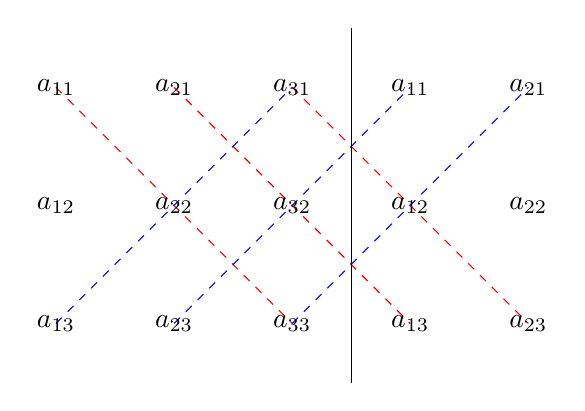
\begin{tikzpicture}
   \begin{scope}[yscale=-1.5,xscale=1.5]
   \draw[color=red,style=dashed]
     (1,1) -- (3,3) (2,1) -- (4,3) (3,1) -- (5,3);
   \draw[color=blue,style=dashed]
     (1,3) -- (3,1) (2,3) -- (4,1) (3,3) -- (5,1);
   \draw(1,1) node {$a_{11}$};
   \draw(1,2) node {$a_{12}$};
   \draw(1,3) node {$a_{13}$};
   \draw(2,1) node {$a_{21}$};
   \draw(2,2) node {$a_{22}$};
   \draw(2,3) node {$a_{23}$};
   \draw(3,1) node {$a_{31}$};
   \draw(3,2) node {$a_{32}$};
   \draw(3,3) node {$a_{33}$};
   \draw(3.5,.5) -- (3.5,3.5);
   \draw(4,1) node {$a_{11}$};
   \draw(4,2) node {$a_{12}$};
   \draw(4,3) node {$a_{13}$};
   \draw(5,1) node {$a_{21}$};
   \draw(5,2) node {$a_{22}$};
   \draw(5,3) node {$a_{23}$};
   \end{scope}
 \end{tikzpicture}
\end{center}
\end{enumerate}

\subsection*{Exercício 8}

  Let $A$ be a square matrix of size $n$.
\begin{enumerate}
\item Calculate $\det A$ for $A = 0_n$ and $A=I_n$.
\item Show that for any scalar $\lambda$, $\det(\lambda A) = \lambda^n \det A$.
  What about $\det B$ where $B$ is obtained by multiplying the coefficients
  of a row $1 \leq i_0 \leq n$ by $\lambda$ that is
  $b_{i_0,j} = \lambda a_{i_0,j}$ for all $1 \leq j \leq n$ and
  $b_{i,j} = a_{i,j}$ for all $i \neq i_0$ and $1 \leq j \leq n$?
  Same question if we multiply only one column of $A$ by $\lambda$.
\item Given a permutation $\sigma$, we define a function $\sigma^{-1}$
  as follows: for any $1 \leq i \leq n$, $\sigma^{-1}(i)$ is the unique
  $1 \leq j \leq n$ such that $\sigma(j) = i$. Clearly, $\sigma^{-1}$ is a
  permutation and ${(\sigma^{-1})}^{-1} = \sigma$.
  Show that
  $\epsilon(\sigma^{-1}) = \epsilon(\sigma)$ and
  $S_n = \{ \sigma^{-1} : \sigma \in S_n \}$. Deduce $\det(A^T) = \det A$.
\item If $A$ is diagonal, prove that
  $\prod_{i=1}^n a_{i,\sigma(i)} \neq 0$ only if $\sigma$ is the identity. Deduce
  $$ \det(A) = \prod_{i=1}^n a_{ii}$$
  If $A$ is only lower triangular, prove that
  $\prod_{i=1}^n a_{i,\sigma(i)} \neq 0$ implies $\sigma(i) \leq i$
  for all $1 \leq i \leq n$. Deduce again that $\sigma$ must be the identity
  and so the same formula holds.
  What about the case when $A$ is upper triangular?
\end{enumerate}

\subsection*{Exercício 9}
We consider a parallelogram given by the points $(0,0)$, $(x_1, y_1)
\neq (0,0)$,
$(x_2,y_2) \neq (0,0)$ and
$(x_1+x_2, y_1+y_2)$. Let $a, b$ be the length of the sides of
the parallelogram and $\gamma$ its internal angle at vertex $(0,0)$.

\begin{enumerate}
\item Use the law of Coseno to express $S = a b \cos \gamma$
  in function of $x_1, x_2, y_1, y_2$.
\item Show that the area $\mathscr A$ of the parallelogram is given by
  ${\mathscr A}^2 = a^2b^2 - S^2$.
\item Conclude that $\mathscr A = \left| \det A \right|$ where
  $A = \begin{pmatrix}
  x_1 & x_2 \\ y_1 & y_2 \end{pmatrix}$.

\item If $A$ is invertible,
  show that any vector $\begin{pmatrix} x \\ y \end{pmatrix}$
  can be expressed as
  $$\begin{pmatrix} x \\ y \end{pmatrix} =
  {u \begin{pmatrix} x_1 \\ y_1 \end{pmatrix}} +
  {v \begin{pmatrix} x_2 \\ y_2 \end{pmatrix}}$$ where
  $$\begin{pmatrix} u \\ v \end{pmatrix} = A^{-1}
  \begin{pmatrix} x \\ y \end{pmatrix}$$
\item What can you say when $A$ is not invertible?
\end{enumerate}

\subsection*{Exercício 10}

Let $A$ and $B$ be two square matrix of dimension $n$.

\begin{enumerate}
\item Recall the expression of the coefficient of the product $AB$ at
  coordinate $1 \leq i,j \leq n$.
\item Deduce that $\det(AB) =
  \sum_{1\leq k_1,k_2,k_3,\dots,k_n\leq n} T_{k_1,k_2,\dots,k_n}$ where
  $$T_{k_1,k_2,\dots,k_n} =
  \left(\prod_{i=1}^n a_{i,k_i}\right)\left(
  \sum_{\sigma \in S_n} \epsilon{(\sigma)}
  {\prod_{i=1}^n b_{k_i,\sigma(i)}}\right)
  $$
\item For any $\tau \in S_n$,
  prove that $S_n = \{ \sigma \circ \tau : \sigma \in S_n \}$.

\item  Consider $1\leq k_1,k_2,k_3,\dots,k_n\leq n$ and suppose there are two
  indices $1 \leq i_1,i_2 \leq n$ such that $k_{i_1} = k_{i_2}$.
  Apply the result of the third question to the
  permutation $\tau_{i_1,i_2} \in S_n$ exchanging $i_1,i_2$ in order
  to prove that $T_{k_1,k_2,\dots,k_n} = -T_{k_1,k_2,\dots,k_n} = 0$.

\item Deduce $\det(AB) = \sum_{\tau \in S_n} T_{\tau(1), \tau(2), \dots, \tau(n)}$.

\item For any $\tau \in S_n$, use the third question to prove that
  $$T_{\tau(1), \tau(2), \dots, \tau(n)} =
  \epsilon{(\tau)}
     \left(\prod_{i=1}^n a_{i,\tau{(i)}}\right)
  \left(\sum_{\sigma \in S_n}
     \epsilon{(\sigma)}
     {\prod_{i=1}^n b_{i,\sigma(i)}}\right)
     $$

\item Conclude that $\det(AB) = \det(A) \det(B)$.

\end{enumerate}

\subsection*{Exercício 11}

\begin{enumerate}
\item Use $I_2 = \begin{pmatrix} 1 & 0 \\ 0 & 0 \end{pmatrix}
  + \begin{pmatrix} 0 & 0 \\ 0 & 1 \end{pmatrix}$ as a counterexample
  for $\det{(A+B)} = \det{(A)} + \det{(B)}$.
\item Let $D$ be a diagonal matrix with diagonal coefficients
  $\lambda_1, \lambda_2, \dots, \lambda_n$. When is $D$ invertible?
  What is the comatrix of $M$? The inverse of $D$?
\item Let $A = \begin{pmatrix}
  a & b & c \\
  d & e & f \\
  g & h & i \end{pmatrix}$.
  Use Laplace's formula to expand
  $\det{(A)}$ along the first column and obtain
  a sum of three determinants of dimension $2$.
  Do the same by expanding $\det{(A)}$ along the second row.
  Simplify the $2$-dimensional determinants and verify that you recover
  the rule of Sarrus.
\item We consider the matrix
  $A = \begin{pmatrix}
  1 & 0 & 1 & 1 \\
  1 & 0 & -1 & 1 \\
  1 & -2 & 1 & -1 \\
  1 & 0 & -1 & -1 \end{pmatrix}$. Prove that
  $\det{(A)} = 2 \begin{vmatrix}
  1 & 1 & 1 \\
  1 & -1 & 1 \\
  1 & -1 & -1 \end{vmatrix}$ and deduce the value of $\det{(A)}$.
\end{enumerate}

\subsection*{Exercício 11}

\begin{enumerate}
\item $\det{I_2} = 1$ but
  the determinants of
  $\begin{pmatrix} 1 & 0 \\ 0 & 0 \end{pmatrix}$ and
  $\begin{pmatrix} 0 & 0 \\ 0 & 1 \end{pmatrix}$ are zero.
\item $\det{(D)} = \prod_{i=1}^n \lambda_i \neq 0$ iff all the
  $\lambda_i \neq 0$ for all $1 \leq i \leq n$.
  The minor $m_{i_0,j_0}$ is obtained by computing the determinant of the matrix
  obtained by removing the $i_0$-th row and the $j_0$-th column. If $i_0 = j_0$,
  we obtain the diagonal matrix with the coefficient $\lambda_{i_0}$ removed
  and so $m_{i_0,i_0} = \prod_{i \neq i_0}^n \lambda_i$.
  If $i_0 \neq j_0$ we obtain a triangular matrix such that at least the
  $\min{i_0,j_0}$-th diagonal coefficient is zero and so
  $m_{i_0,j_0} = 0$. Finally, $M$ is a diagonal matrix
  such that the $i_0$-th diagonal coefficient is
  ${(-1)}^{i_0+i_0} m_{i_0,i_0} = \prod_{i \neq i_0}^n \lambda_i$.
  In particular, $M^T = M$ and if $D$ is invertible
  $D^{-1} = \frac{1}{\det{D}} M^T$ is the diagonal matrix such that
  the $i$-th diagonal coefficient is $\lambda_i^{-1}$.
\item If we expand along the first column we obtain
  $$\det{(A)} =
  \begin{vmatrix} a & b & c \\ d & e & f \\ g & h & i \end{vmatrix} =
  {a \begin{vmatrix} e & f \\ h & i \end{vmatrix}}
  - {d \begin{vmatrix} b & c \\ h & i \end{vmatrix}}
  + {g \begin{vmatrix} b & c \\ e & f \end{vmatrix}}$$
  If we expand along the second row we obtain
  $$\det{(A)} =
  \begin{vmatrix} a & b & c \\ d & e & f \\ g & h & i \end{vmatrix} =
  - {d \begin{vmatrix} b & c \\ h & i \end{vmatrix}}
  + {e \begin{vmatrix} a & c \\ g & i \end{vmatrix}}
  - {f \begin{vmatrix} a & b \\ g & h \end{vmatrix}}$$
  The first one becomes
  $a{(ei - fh)} - d{(bi - ch)} + g{(bf - ce)}=
  aei + bfg + cdh - gec - hfa - idb$ which is the expression given by
  the rule of Sarrus. This is similar for the second one.

\item We consider the matrix
  If we expand the determinant of $A$ along the second column, then
  the only nonzero term in Laplace's formula
  is the one for $(i,j) = (3,2)$ which is
  ${(-1)}^5 \times {(-2)} \begin{vmatrix}
  1 & 1 & 1 \\
  1 & -1 & 1 \\
  1 & -1 & -1 \end{vmatrix}$.
  Using the rule of Saarus, we deduce that
  $\det{(A)} = 2 \times \left(1 + 1 - 1 + 1 + 1 + 1\right) = 8$.
\end{enumerate}

\section{Resolução e discussão de sistemas lineares}

Let $n, m$ be natural numbers. We consider numbers
$a_{i,j}$ and $b_i$ for $1 \leq i \leq n$ and $1 \leq j \leq m$.
Then a sistema lineare is a set of equations
%%
$$\begin{aligned}
    a_{11} x_1 + a_{12} x_2 + \dots + a_{2m} x_m &= b_1 \\
    a_{21} x_1 + a_{22} x_2 + \dots + a_{2m} x_m &= b_2 \\
    \dots \\
    a_{n1} x_1 + a_{n2} x_2 + \dots + a_{nm} x_m &= b_n
  \end{aligned}$$
%%
with unknowns $x_1, x_2, \dots, x_m$. If $A$ is the $n$-by-$m$
matrix of coefficients $a_{ij}$,
$x$ the column vector with $m$ coefficients $x_j$ and
$b$ the column vector with $n$ coefficients $b_i$ then this is equivalent to
the matrix equation
%%
$$Ax = b$$
%%
with unknown $x$. Note that if $n = m$ then $A$ is a square matrix.
If $A$ is invertible then $x = A^{-1} b$ is the unique solution.

Suppose first that $a_{i1} = 0$ for all $1 \leq i \leq n$. These are the
coefficients in front of $x_1$ so we can set $x_1$ to an arbitrarily value
without changing the set of equations and the problem is reduced to a system
with $m-1$ unknowns.
Otherwise, we can assume that $a_{11} \neq 0$ (if necessary by exchanging
the first and $i$-th equation to ensure that) and for each $1 < i \leq n$, we
substract $\frac{a_{i1}}{a_{11}}$ times the first equation from the $i$-th
equation. We obtain an equivalent system where all the coefficients in front
of $x_1$ are zero, except for the first equation.

Now suppose that $a_{11} \neq 0$ and $a_{i1} = 0$ for all $i > 1$. If
$a_{i2} = 0$ for all $2 \leq i \leq n$ then we can
set $x_2$ to an arbitrarily value and we obtain a new system with
$m-1$ unknowns such that all the coefficients in front of $x_1$ are zero,
except for the first equation.
Otherwise, we can assume that $a_{22} \neq 0$ (if necessary by exchanging
the second and $i$-th equation to ensure that) and for each $1 < i \leq n$, we
substract $\frac{a_{i2}}{a_{22}}$ times the first equation from the $i$-th
equation. We obtain an equivalent system where all the coefficients in front
of $x_2$ are zero, except for the first and second equations.

Continuing like this, we can reduce the problem to a triangular system of
$n$ equations and $m'$ unknowns
%%
$$A'x' = b'$$
%%
where $A'$ is upper triangular ($a'_{ij} = 0$ if $i > j$)
such that all the diagonal coefficients $a'_{ii} \neq 0$. We have three cases:
\begin{enumerate}
\item If $n = m'$, then $\det{A'} \neq 0$
  and in that case there is a unique solution $x' = {(A')}^{-1} b'$.
\item If $n > m'$ then the $i$-equations for $m' < i \leq n$ are
  $0 = b'_i$. If they are not satisfied, the system does not have any solution.
  Otherwise, we only need to consider $i$-equations for $1 \leq i \leq m'$ and
  so we come back to the case $n = m'$.
\item If $n < m'$ then the last equation is
  $a'_{n,n} x'_{n} + a'_{n,{(n+1)}} x'_{n+1} + \dots + a'_{n,m'} x'_{m'} = b'_{n}$.
  We can
  then arbitrarily fix $x'_{n+1}, x'_{n+2}, \dots, x'_{m'}$ and thus again
  go back to the case $n = m'$.
\end{enumerate}

The previous algorithm is known as Gaussian elimination. It can actually be
interpreted as an algorithm on a matrix $A$, as a repetition of operations
among:

\begin{enumerate}
\item Swapping two rows $L_i \leftrightarrow L_j$.
\item Multiplying a row by a non-zero scalar $L_i \leftarrow \lambda L_i$.
\item Adding a multiple of one row to another row
  $L_i \leftarrow L_i + \lambda L_j$.
\end{enumerate}

At the end of the Gaussian Elimination for systems of linear equations
we obtain a triangular system that can then easily be solved. Similarly, in the
matrix form, we obtain an upper triangular matrix. One can check that the first
operation multiplies the determinant of the matrix by $-1$, the second
multiplies the determinant by the same scalar and the third does not change the
determinant. Finally, the determinant of the triangular matrix obtained at the
end can easily be computed as the product of the diagonal coefficients and
hence we can deduce the determinant of the initial matrix $A$.

In the Gaussian Elimination for systems of linear equations we can even
go further by subtracting multiples of the last row from the rows above
in order to eliminate one variable in these rows ; and recursively
eliminate more variables in the upper rows.
In matrix term, this is obtaining the reduced row echelon form:

\begin{enumerate}
  \item All nonzero rows are above any zero rows.
  \item The pivot of a nonzero row (the first nonzero number from the left)
    is always 1.
  \item The pivot of a nonzero row is strictly to the right of
    pivots of the rows above it.
  \item The pivot of a nonzero row is the only nonzero entry in its column.
\end{enumerate}

Here is a typical example for a 5-by-5 matrix. The pivots are painted
in red. Note that there is
no way to apply row operations in order to "eliminate" the non-pivot
coefficients any further.
    $$
    \begin{pmatrix}
    \color{red} 1 & -5 & 0 & 3 & 0 \\
    0 & 0  & \color{red} 1 & 1 & 0 \\
    0 & 0  & 0 & 0  & \color{red} 1 \\
    0 & 0 & 0  & 0 & 0 \\
    0 & 0 & 0  & 0 & 0
    \end{pmatrix}$$

If the initial matrix $A$ is a square matrix and we obtain the reduced row
echelon form, then $A$ is invertible if and only if
the reduced row echelon form is the identity $I_n$. A way to
invert a matrix is then to apply the same row operations to
$I_n$. Typically, we place $I_n$ next to
the matrix we want to invert as below. We then do the
Gaussian Elimination on the left hand side matrix and apply the same
row operations on the right hand side matrix.

\subsection*{Exercício 11}

Solve the following systems using Gaussian elimination:

\begin{enumerate}

\item $$\left\{\begin{aligned}-3x-5y&=69\\-4x+7y&=-31\end{aligned}\right.$$
\item $$\left\{\begin{aligned}-6x-3y-2z&=20\\-3x+3y+z&=59\\-7x-5y+7z&=27\end{aligned}\right.$$
\item
  $$\left\{\begin{aligned}-x-5y-6z-4v&=-21\\x+4y+5z-6v&=-10\\-5x-3y-6z+2v&=-27\\4x-3y-4z-3v&=29\end{aligned}\right.$$

\end{enumerate}

\subsection*{Exercício 12}

Let $A = \begin{pmatrix}
          1 & 2 & 0 & 0   \\
          -1 & 8 & 9 & 7 \\
          0 & 5 & 0 & 3   \\
          1 & 0 & 0 & -1  \\
      \end{pmatrix}$. Calculate the minor $m_{2 3}$ using the rule of Sarrus.
Now use Laplace's formula for $j=3$ to deduce $\det{(A)}$.
Determine the triangular matrix $B$ obtained from the following operations:
$L_2 \leftarrow L_2 + L_1$, $L_4 \leftarrow L_4 - L_1$,
$C_2 \leftrightarrow C_3$, $L_3 \leftarrow L_3 / 5$,
$L_4 \leftarrow L_4 + 2 L_3$. Compute $\det{(B)}$ and compare with
$\det{(A)}$.

\subsection*{Exercício 13}

Use Gaussian Elimination to determine the inverse of
%%
$A = \begin{pmatrix}
  1 & 0 & -2 & -1 & 0   \\
  -4 & 0 & 0 & 0 & 4 \\
  4 & 4 & -7 & -7 & 1   \\
  -3 & 1 & 1 & 0 & 3  \\
  -5 & 2 & 2 & 1 & 5
\end{pmatrix}$.
Use $A^{-1}$ to deduce the solution of the following linear
system of 5 equations and 5 unknowns:
%%
$$
A \begin{pmatrix} x_1 \\ x_2 \\ x_3 \\ x_4 \\ x_5 \end{pmatrix} =
\begin{pmatrix} 4 \\ 8 \\ 12 \\ 16 \\ 20 \end{pmatrix}
$$

\section{Solução do Exercícios}

\subsection*{Exercício 1}

\begin{enumerate}

\item Square diagonal matrix with dimension $n = m = 3$. The coefficients are
  $a_{ij} = 0$ for all $1 \leq i \neq j \leq 3$ and
  $a_{ii} = \frac{i}{2}$ for all $1 \leq i \leq 3$.

\item Upper triangular matrix with dimension $n = 4$ and $m=5$.
  The coefficients are
  $b_{ij} = 0$ if $1 \leq j < i \leq 4$ and
  $b_{ij} = 1$ if $1 \leq i \leq 4$ and $i \leq j \leq 5$.

\item Lower triangular square matrix with dimension $n = m = 4$.
  The coefficients are
  $c_{ij} = 0$ if $1 \leq i < j \leq 4$,
  $c_{ii} = i$ if $1 \leq i \leq 4$ and
  $c_{ij} = {(-1)}^{i+j}$ if $1 \leq j < i \leq 4$.

\item Matrix with dimension $n = 4$ and $m = 3$.
  The coefficients are
  $d_{ij} = i + j$ for all $1 \leq i \leq 4$ and $1 \leq j \leq 3$.
  Not that it is not symmetric because $n \neq m$.
\item Antisymmetric matrix with dimension $n = m = 3$.
  The coefficients are
  $e_{ij} = j$ and $e_{ji} = -e_{ij} = -j$
  for all $1 \leq i < j \leq 4$ and
  $e_{ii} = 0$ for all $1 \leq i \leq 4$.
\end{enumerate}

\subsection*{Exercício 2}
\begin{enumerate}
\item Not defined: the two matrices do not have the same dimension.
\item $\begin{pmatrix}
  6 & -4 & 2 \\
  4 & 1 & 10 \\
\end{pmatrix}$
\item $\begin{pmatrix}
  19 & 5 \\
  5 & 9
\end{pmatrix}$
\item $-\begin{pmatrix}
  -8 & -3 & -4 \\
  -3 & -4 & -9 \\
  -5 & 0 & -2 \\
  -11 & -4 & 0
\end{pmatrix}$

\end{enumerate}

\subsection*{Exercício 3}

\begin{enumerate}
\item Not defined: $A$ has 3 colums and $B$ 2 rows.
\item $BA = \begin{pmatrix}
  1 & 2 & 3 \\
  7 & 15 & 21
\end{pmatrix}$
\item $BB = B^2 = I_2 = \begin{pmatrix}
  1 & 0 \\
  0 & 1\end{pmatrix}$
\item $BC = \begin{pmatrix}
  0 & 0 \\
  -1 & 0\end{pmatrix} \neq \begin{pmatrix}
  0 & 0 \\
  1 & 0\end{pmatrix} = CB$
\item $CC = C^2 = 0_2 = \begin{pmatrix}
  0 & 0 \\
  0 & 0\end{pmatrix}$

\item $DE =
  \begin{pmatrix}
  \lambda_1 a & \lambda_1 b & \lambda_1  c \\
  \lambda_2 d & \lambda_2 e & \lambda_2 f  \\
  \lambda_3 g & \lambda_3 h & \lambda_3 i  \end{pmatrix}$
  and
  $ED =
  \begin{pmatrix}
  \lambda_1 a & \lambda_2 b & \lambda_3  c \\
  \lambda_1 d & \lambda_2 e & \lambda_3 f  \\
  \lambda_1 g & \lambda_2 h & \lambda_3 i  \end{pmatrix}$.
\end{enumerate}


\subsection*{Exercício 4}

\begin{enumerate}
\item When $n = m = 1$, the Hadamard product becomes
  ${(a_{11})} \times {(b_{11})} = {(a_{11}b_{11})}$. This is the standard
  product of matrices and corresponds to the product of numbers.
\item Given three $n$-by-$m$ matrices $A, B, C$ we have
  for $1 \leq i \leq n$ and $1 \leq j \leq m$:
  ${(a_{i,j} b_{i,j})} c_{i,j} = a_{i,j} {(b_{i,j} c_{i,j})}$,
  ${(a_{i,j} + b_{i,j})} c_{i,j} = {(a_{i,j}c_{i,j})} + {(b_{i,j}c_{i,j})}$ and
  $a_{i,j} b_{i,j} = b_{i,j} a_{i,j}$. Hence
  ${(A \times B)} \times C = A \times {(B \times C)}$,
  ${(A+B)}\times C = {A\times C} + {B\times C}$ and
  $A\times B = B\times A$.
\item This is because
  $a_{i,j} 0 = 0 a_{i,j} = 0$ for $1 \leq i \leq n$ and $1 \leq j \leq m$.
\item Similarly, if we consider a $n$-by-$m$ matrix $I$ with all coefficients
  that are $1$'s then
  $a_{i,j} 1 = 1 a_{i,j} = 1$ for $1 \leq i \leq n$ and $1 \leq j \leq m$
  and so $A \times I = I \times A = A$.
\item For any $n$-by-$m$ matrices $A, B$ we have
  $A B = I$ iff $B A = I$ iff
  $a_{i,j} b_{i,j} = 1$ for all $1 \leq i \leq n$ and $1 \leq j \leq m$.
  So given $A$, such matrix $B$ exists iff
  all coefficients of $A$ are nonzero and then $b_{i,j} = \frac{1}{a_{i,j}}$
  for all $1 \leq i \leq n$ and $1 \leq j \leq m$.
\item $(x,y) = ({1x+0y}, {0x+1y})$ so the identity is
  $L_{1,0,0,1}$.
\item $L_{1,0,0,-1}: (2,1) \mapsto (2,-1)$,
  $L_{1,0,0,-1}: (-1,3) \mapsto (-1,-3)$,
  $L_{0,-1,1,0}: (2,1) \mapsto (-1,2)$,
  $L_{0,-1,1,0}: (-1,3) \mapsto (-3,-1)$.
  This suggests that $L_{1,0,0,-1}$ is the symmetric with respect to the $x$-axis
  and $L_{0,-1,1,0}$ the rotation of angle $90°$ around the origin.
\begin{center}
  \begin{tikzpicture}
    \draw[->] (-4,0) -- (4,0) node[above] {$x$};
    \draw[->] (0,-4) -- (0,4) node[right] {$y$};
    \foreach \i in {-3,-2,-1,1,2,3} {
      \draw(\i,-.1) -- (\i,.1) node[above right]{$\i$};
      \draw(-.1,\i) -- (.1,\i) node[above right]{$\i$};
    }
    \draw[style=dashed,color=red] (-1,3)
    arc(108.434948822922:198.434948822922:3.162277660168379);

    \draw [style=dashed,color=blue] (2,1)
    arc(26.56505117707799:116.5650511770779:2.23606797749979);

    \draw[style=dashed,color=red] (-1,3) -- (-1,-3);
    \draw[style=dashed,color=blue] (2,1) -- (2,-1);

    \fill[color=blue] (2,1) circle(.1) node[right]{$(2,1)$};
    \fill[color=blue] (2,-1) circle(.1) node[right]{$(2,-1)$};
    \fill[color=blue] (-1,2) circle(.1) node[left]{$(-1,2)$};

    \fill[color=red] (-1,3) circle(.1) node[left]{$(-1,3)$};
    \fill[color=red] (-1,-3) circle(.1) node[left]{$(-1,-3)$};
    \fill[color=red] (-3,-1) circle(.1) node[left]{$(-3,-1)$};
\end{tikzpicture}
\end{center}

\item
  $L_{0,-1,1,0}: (x,y) \mapsto (-y,x)$ and
  $L_{0,1,-1,0}: (-y,x) \mapsto (x,y)$ so $L_{0,1,-1,0} \circ L_{0,-1,1,0}$ is
  the identity $(x,y) \mapsto (x,y)$. Similarly,
  $L_{0,1,-1,0} \circ L_{0,-1,1,0} = L_{0,-1,1,0} \circ L_{0,1,-1,0} = L_{1,0,0,1}$
  Hence $L_{0,-1,1,0}$ is invertible with inverse
  $L_{0,1,-1,0}$. The previous question suggested the invertibility of
  $L_{0,-1,1,0}$ and that
  the inverse is the rotation of angle $-90°$ around the origin.

\item
  We have $L_{1,0,0,-1}: (x,y) \mapsto (x,-y)$
  and $L_{0,-1,1,0}: (x,-y) \mapsto (y,x)$.
  We also have $L_{0,-1,1,0}: (x,y) \mapsto (-y,x)$ and
  $L_{1,0,0,-1}: (-y,x) \mapsto (-x,-y)$.
  So $L_{1,0,0,-1} \circ L_{0,-1,1,0} \neq L_{0,-1,1,0} \circ L_{1,0,0,-1}$.
  This is again expected by the analogy with geometric transformations.
  For example base the vector $\vec{i}=(1,0)$ is not moved by the $x$-axis
  symmetry and then moved to the base vector $\vec{j}=(0,1)$ by the rotation of
  90°. However we get a different result if we permute the transformation:
  the $\vec{i}$ is moved to $\vec{j}$ by the rotation of 90° and
  then moved to $-\vec{j}$ by the $x$-axis symmetry. So the $x$-axis symmetry
  and rotation of 90° do not commute.
\item
  $L_{a,b,c,d}: (x,y) \mapsto {(ax+by,cx+dy)}$
  and $$L_{e,f,g,h}: {(ax+by,cx+dy)} \mapsto
  {({e(ax+by)+f(cx+dy)}, {g(ax+by)+h(cx+dy)})}$$
%%
  Hence we obtain
  $$L_{e,f,g,h} \circ L_{a,b,c,d} = L_{ea+fc,eb+fd,ga+hc,gb+hd}$$
  This is in general different from the pairwise
  product of coefficient $L_{ea,fb,gc,hd}$ but we recognize the coefficient
  of the matrix product
  $$
  \begin{pmatrix}
       e & f \\
       g & h
  \end{pmatrix}
  \begin{pmatrix}
       a & b \\
       c & d
  \end{pmatrix} =
  \begin{pmatrix}
       ea+fc & eb+fd \\
       ga+hc & gb+hd
  \end{pmatrix}
$$
\end{enumerate}

\subsection*{Exercício 5}

\begin{enumerate}
\item $\begin{pmatrix}
      2 & 8  \\
      4 & 10  \\
      6 & 12
\end{pmatrix}$
\item $XYZ = \begin{pmatrix}
      12 & 14  \\
      24 & 28
\end{pmatrix}$, $YXZ = \begin{pmatrix}
      39 & 48  \\
      13 & 16
\end{pmatrix}$ and $ZXY = \begin{pmatrix}
      -11 & 33  \\
      -17 & 51
\end{pmatrix}$. They have respective trace $12+28=40$, $39+16=55$ and
  $-11+51=40$.
\item We consider a one $m$-by-$n$ matrix $A$ and one $n$-by-$p$ matrix $B$.
  Then $C=AB$ is a well defined $m$-by-$p$ matrix with coefficient
  $c_{i,j} = \sum_{k=1}^n a_{i,k} b_{k,j}$
  for $1\leq i \leq m$ and $1\leq j \leq p$.
  $A^T$ is an $n$-by-$m$ matrix $A$ and $B$ a $p$-by-$n$ matrix so
  $D=BA$  is a well defined $p$-by-$m$ matrix with coefficient
  $d_{j,i} = \sum_{k=1}^n b_{i,k} a_{k,j}$
  for $1\leq i \leq m$ and $1\leq j \leq p$. Then $D = C^T$.

\item We consider two square matrices $A,B$ of size $n$. Then
  $C=AB$ is a well defined square matrix of size $n$ with coefficient
  $c_{i,j} = \sum_{k=1}^n a_{i,k} b_{k,j}$
  for $1\leq i,j \leq n$. So the trace of $C$ is
  $$\sum_{i=1}^n c_{i,i} = \sum_{i=1}^n {\sum_{k=1}^n a_{i,k} b_{k,i}}$$
  But this double sum remains the same if we exchange the role of $a$ and $b$
  and so $\operatorname{Tr}(A B) = \operatorname{Tr}(B A)$.
\item
  For square matrices $A_1,A_2,\dots,A_k,A_{k+1}$
  of size $n$ we apply the previous formula for $A = A_1 A_2 \dots A_k$ and
  $B = A_{k+1}$.
\end{enumerate}

\subsection*{Exercício 6}
\begin{enumerate}
\item $\begin{pmatrix}
  a & b \\
  c & d
\end{pmatrix} \begin{pmatrix}
  x \\
  y
\end{pmatrix} =
\begin{pmatrix}
  a x + by \\
  c x + d y
\end{pmatrix}$ so $L_{a,b,c,d}(x,y)$ is just obtained by a matrix product.
We recall that the coefficients of
${L_{e,f,g,h}} \circ {L_{a,b,c,d}}$ are also obtained via
the matrix product $\begin{pmatrix}
  e & f \\
  g & h
\end{pmatrix} \begin{pmatrix}
  a & b \\
  c & d
\end{pmatrix}$

\item If $A = \begin{pmatrix}
  a & b \\
  c & d
\end{pmatrix}$ then
  $ A \begin{pmatrix}
  x \\
  y
\end{pmatrix} =
  A \left( x \begin{pmatrix}
  1 \\
  0
\end{pmatrix} + y \begin{pmatrix}
  0 \\
  1
  \end{pmatrix} \right)$ and so
  $$  A \begin{pmatrix}
  x \\
  y
\end{pmatrix} = x \left[A\begin{pmatrix}
  1 \\
  0
\end{pmatrix}\right] + y \left[A\begin{pmatrix}
  0 \\
  1
    \end{pmatrix}\right]$$
  that is
  $$L_{a,b,c,d}(x,y) = x {L_{a,b,c,d}(\vec{i})} + y {L_{a,b,c,d}(\vec{j})}$$

\item We obtain
$D_{\lambda,\mu} \begin{pmatrix}
  x \\
  y
\end{pmatrix} = \begin{pmatrix}
  \lambda x \\
  \mu y
\end{pmatrix}$ so $D_{\lambda,\mu}$ is the diagonal matrix $\begin{pmatrix}
  \lambda & 0 \\
  0 & \mu
\end{pmatrix}
  $ with trace $\lambda+\mu$.

\item For example,
  $\begin{pmatrix}
  \lambda & 0 \\
  0 & \mu
\end{pmatrix} \begin{pmatrix}
  \frac{1}{\lambda} & 0 \\
  0 & \frac{1}{\mu}
\end{pmatrix} = \begin{pmatrix}
  \frac{\lambda}{\lambda} & 0 \\
  0 & \frac{\mu}{\mu}
\end{pmatrix} = I_2$
\item We have $\vec{i} =  \vec{v} - 2\vec{u}$ and
  $\vec{j} = \frac{3\vec{u}-\vec{v}}{2}$.

\item $X\vec{u} +Y\vec{v} = \left(X+3Y\right)\vec{i}
  + \left(2X+4Y\right)\vec{j}$ so its image by $S_{\lambda,\mu}$ is
  $\lambda \left(X+3Y\right)\vec{i} + \mu \left(2X+4Y\right)\vec{j}$ which is
  $\lambda \left(X+3Y\right)\left(\vec{v} - 2\vec{u}\right) +
  \mu \left(X+2Y\right)\left(3\vec{u} - \vec{v}\right)$. We then find
  $$\begin{pmatrix} e & f \\ g & h \end{pmatrix} = \begin{pmatrix}
  2\mu-2\lambda & 6\mu-6\lambda \\
  \lambda-\mu & 3\lambda-\mu
  \end{pmatrix}$$
  and the trace is $e+f=2\mu-2\lambda+3\lambda-\mu=\lambda+\mu$ which is also
  the trace of $D_{\lambda,\mu}$! Note: more generally, we can prove that the
  trace of the matrix of $S_{\lambda,\mu}$ in any base is $\lambda+\mu$.

\item We have
  $R_{\theta} \begin{pmatrix} 1 \\ 0 \end{pmatrix} =
  \begin{pmatrix} \cos{\theta} \\ \sin{\theta} \end{pmatrix}$ and
  $R_{\theta} \begin{pmatrix} 0 \\ 1 \end{pmatrix} =
  \begin{pmatrix} -\sin{\theta} \\ \cos{\theta} \end{pmatrix}$
  so $R_{\theta} \begin{pmatrix} x \\ y \end{pmatrix} =
  \begin{pmatrix} x\cos{\theta} - y\sin{\theta} \\
    x\sin{\theta} + y\cos{\theta}
  \end{pmatrix}$ and
  $$R_{\theta} = \begin{pmatrix} \cos{\theta} & - \sin{\theta} \\
    \sin{\theta} & \cos{\theta}
  \end{pmatrix}$$
\item Using $\sin{(-\theta)} = -\sin \theta$ we find that
  the coefficients of
  $R_{\theta} R_{-\theta}$ and $R_{-\theta} R_{\theta}$
  outside the diagonal are zero.
  Moreover using $\cos^2{\theta} + \sin^2{\theta} = 1$ we find that
  the diagonal coefficients are $1$.
  More generally, we find $R_{\theta_1} R_{\theta_2} = R_{\theta_1 + \theta_2}$
  using the expressions of $\cos{(\theta_1+\theta_2)}$ and
  $\sin{(\theta_1+\theta_2)}$ from Bimestre 1.
\item We find $D_{\lambda,\mu}^T = D_{\lambda,\mu}$ and
  $R_{\theta}^T = R_{-\theta}$.
\item We indeed find
  $\begin{pmatrix} x \\ y \end{pmatrix}^T \begin{pmatrix} x \\ y \end{pmatrix} =
  \begin{pmatrix} x & y \end{pmatrix} \begin{pmatrix} x \\ y \end{pmatrix}
  = {(x^2 + y^2)} = {(\alpha)}$.
\item If $A$ is the matrix of a linear transformation such that
  $A^T A = I_2$ then for any vector $v$ we have
  ${(Av)}^T {(Av)} = v^T A^T A v = v^T I_2 v = v^T v$ so by the previous question
  $Av$ and $v$ have the same norm.
\item For any $\theta$ we have
  $R_{\theta}^T R_\theta = R_{-\theta} R_{\theta} = I_2$ and indeed rotations
  preserve the norm of vectors.
  We have $D_{\lambda,\mu}^T D_{\lambda,\mu} = D_{\lambda,\mu}^2 =
  \begin{pmatrix} \lambda^2 & 0  \\ 0 & \mu^2 \end{pmatrix} =
  I_2$ iff $\lambda^2 = 1$ and $\mu^2 = 1$. So this happens in four cases,
  all of obviously them preserving the norm of vectors:
  $D_{1,1}= \begin{pmatrix} 1 & 0 \\ 0 & 1 \end{pmatrix}$ (identity),
  $D_{-1,1}=\begin{pmatrix} -1 & 0 \\ 0 & 1 \end{pmatrix}$ (symmetry with respect to the $x$-axis),
  $D_{1,-1}=\begin{pmatrix} 1 & 0 \\ 0 & -1 \end{pmatrix}$ (symmetry with respect to the $y$-axis),
  $D_{-1,-1} = R_{\pi} = \begin{pmatrix} -1 & 0 \\ 0 & -1 \end{pmatrix}$
  (symmetry with respect to the origin, that is rotation of 180° around
  the origin).
\end{enumerate}

\subsection*{Exercício 7}

\begin{enumerate}
\item For $n=1$,
  the unique permutation of $X_n = \{ 1 \}$ is $\sigma: 1 \mapsto 1$ product
  which has signature 1. Hence $\det(A) = a_{11} = \alpha$ and
  $\det(A) \neq 0$ iff $\alpha \neq 0$. In that case, the comatrix of $A$
  is $M = (m_{11}) = (1)$ and $A^{-1} = \frac{1}{\alpha} M^T = {(\alpha^{-1})}$.
  This is the same as for real numbers:
  $\alpha$ is invertible iff $\alpha \neq 0$ and in that case $\alpha^{-1}$
  satisfies (by definition) $\alpha \alpha^{-1} = \alpha^{-1} \alpha = 1$.
\item  For $n=2$ there are two permutations to consider: the identity of $X_2$
  (giving the term $a_{11}a_{22}=ac$ in the expression of the determinant)
  and the transposition $(12)$ (giving the term $-a_{12}a_{21}=-bd$). Hence
  $\det(A) =  ad - bc$. The comatrix of $A$ is
  $M = \begin{pmatrix} d & -c \\ -b & a \end{pmatrix}$.
  If $ad - bc \neq 0$
  then $B = \frac{1}{ad - bc} \begin{pmatrix} d & -b \\ -c & a \end{pmatrix}$.
  We verify $AB = \frac{1}{ad - bc}
  \begin{pmatrix} ad - bc & cd - dc \\ -ab + ba & -bc + ad \end{pmatrix} = I_2$.
\item From the rule of Sarrus we obtain:
  $$\det(A) = a_{11}a_{22}a_{33}+a_{12}a_{23}a_{31}+a_{13}a_{21}a_{32}-a_{31}a_{22}a_{13}-a_{32}a_{23}a_{11}-a_{33}a_{21}a_{12}$$
  In the general definition of determinant, these 6 terms correspond
  to following permutations:
  the identify, $(1,2) \circ (2,3)$,
  $(1,3) \circ (2,3)$, $(1,3)$, $(2,3)$ and $(1,2)$.
  For $n=2$, a similar rule holds:
  From the products of the diagonal
  going from top to bottom ($a_{11}a_{22}$), substract the products of the
  diagonal going from bottom to top ($a_{21}a_{12}$).
\begin{center}
  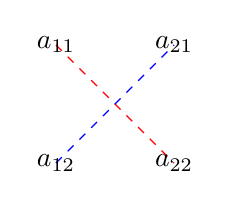
\begin{tikzpicture}
   \begin{scope}[yscale=-1.5,xscale=1.5]
   \draw[color=red,style=dashed] (1,1) -- (2,2);
   \draw[color=blue,style=dashed] (1,2) -- (2,1);
   \draw(1,1) node {$a_{11}$};
   \draw(1,2) node {$a_{12}$};
   \draw(2,1) node {$a_{21}$};
   \draw(2,2) node {$a_{22}$};
   \end{scope}
 \end{tikzpicture}
\end{center}

\end{enumerate}

\subsection*{Exercício 8}
\begin{enumerate}
\item For $A=0_n$, all the coefficients $a_{i, \sigma(i)}$ are zeros
  so $\det A = 0$.
  The determinant of $I_n$ can be expressed using Kronecker's delta:
%%
  $$\sum_{\sigma \in S_n} \epsilon(\sigma) \prod_{i=1}^n {\delta_{i,\sigma(i)}}$$
%%
  If $\sigma$ is not the identity, then for some $1 \leq i \leq n$ we have
  $\sigma(i) \neq i$ and so $\delta_{i,\sigma(i)} = 0$ ; a fortiori,
  $\prod_{i=1}^n {\delta_{i,\sigma(i)}} = 0$. The term corresponding to the identity
  permutation is $1$ so $\det(I_n) = 1$.
\item The determinant of $\lambda A$ is defined by
%%
  $$\sum_{\sigma \in S_n} \epsilon(\sigma) \prod_{i=1}^n {\lambda a_{i,\sigma(i)}}$$
%%
  and we see that we can factor out $\lambda^n$ to obtain
  $\det(\lambda A) = \lambda^n \det A$.
  If $B$ is obtained by multiplying only
  the coefficients of the $i_0$-th row by $\lambda$,
  then for all $\sigma \in S_n$ we have
  $\prod_{i} {b_{i,\sigma(i)}} = \prod_{i \neq i_0} {a_{i,\sigma(i)}} \times
  {(\lambda a_{i_0,\sigma(i_0)})}$ so we can factor out one $\lambda$ and
  $\det B = \lambda \det A$. If $C$ is obtained by multiplying only the
  $j_0$-th column then
  for each $\sigma \in S_n$, a factor $\lambda$ will only appear for the unique
  $i$ such that $\sigma(i) = j_0$ and so again $\det C = \lambda \det A$.
\item Let $\sigma, \tau \in S_n$ such that $\sigma \neq \tau$. Then there is
  $i$ such that $\sigma{(i)} \neq \tau{(i)}$
  and so $\tau^{-1}{(\sigma{(i)})} \neq \tau^{-1}{(\tau{(i)})}$. But by
  definition, ${\tau^{-1}{(\tau{(i)})}} =  i = {\sigma^{-1}{(\sigma{(i)})}}$.
  Hence $\tau^{-1} \neq \sigma^{-1}$
  and $\{ \sigma^{-1} : \sigma \in S_n \}$ enumerates the $n!$ elements of $S_n$.
  $\sigma \circ \sigma^{-1}$ is the identity so
  $\epsilon(\sigma) \epsilon(\sigma^{-1}) = 1$ and
  $\epsilon(\sigma^{-1}) = \epsilon(\sigma)$.
  The determinant of $A^T$ is
%%
  $$\sum_{\sigma \in S_n} \epsilon(\sigma) \prod_{i=1}^n {a_{\sigma(i),i}}$$
%%
  By definition $ \{ 1, 2, 3, \dots, n \} =
  \{ \sigma^{-1}{(1)}, \sigma^{-1}{(3)}, \sigma^{-1}{(3)},
  \dots, \sigma^{-1}{(n)} \}$ and so
%%
  $$\prod_{i=1}^n {a_{\sigma(i),i}}=
  \prod_{i=1}^n {a_{\sigma{(\sigma^{-1}(i))},\sigma^{-1}(i)}} =
  \prod_{i=1}^n {a_{i,\sigma^{-1}(i)}}$$
%%
  Since $S_n = \{ \sigma^{-1} : \sigma \in S_n \}$,
  the determinant of $A^T$ becomes
%%
  $$
  \sum_{\sigma \in S_n} \epsilon(\sigma^{-1}) \prod_{i=1}^n {a_{i,{(\sigma^{-1})}^{-1}{(i)}}}$$
  %%
And since ${(\sigma^{-1})}^{-1} = \sigma$ and
$\epsilon{(\sigma^{-1})} = \epsilon(\sigma)$ we finally obtain:
  $$
  \sum_{\sigma \in S_n} \epsilon(\sigma) \prod_{i=1}^n {a_{i,\sigma{(i)}}} =
  \det{(A)}$$
%%

  \item $\prod_{i=1}^n a_{i,\sigma(i)} = 0$ if $a_{i,\sigma(i)} = 0$ for some
    $1 \leq i \leq n$. If $A$ is diagonal this happens
    for if $\sigma(i) \neq i$ for some $1 \leq i \leq n$ that is if
    $\sigma$ is not the identity.
    So the only nonzero term of
    the coefficient is given by the identity $\sigma: i \mapsto i$, which is
    $\prod_{i=1}^n a_{ii}$.

    If $A$ is lower triangular, $a_{i,\sigma(i)} = 0$ happens for all
    $\sigma(i) > i$. Hence $\prod_{i=1}^n a_{i,\sigma(i)} \neq 0$ implies
    $\sigma(i) \leq i$ for all $1 \leq i \leq n$.
    $\sigma(1) \leq 1$ implies that $\sigma(1) = 1$.
    Then $\sigma(2) \neq \sigma(1) = 1$ and $\sigma(2) \leq 2$ so
    $\sigma(2) = 2$. Continuing like this we deduce
    $\sigma(i) = i$ for all $1 \leq i \leq n$. Again, $\sigma$ must be the
    identity and the same formula $\det A = \prod_{i=1}^n a_{ii}$ holds.

    If $A$ is upper triangular, we do the same proof using
    $\sigma(i) \geq i$ for all $1 \leq i \leq n$. We prove
    $\sigma(i) = i$ starting from $i=n$ and going down until $i=1$.
\end{enumerate}

\subsection*{Exercício 9}

\begin{enumerate}
\item
  We consider the triangles given by the points
  $(0,0)$, $(x_1, y_1)$, $(x_2,y_2)$ and $c$ is the length of the side opposite
  to $\gamma$.
  The law of Coseno is
  $$c^2 = a^2 + b^2 - 2ab\cos\gamma$$
  where
  $a^2 = x_1^2 + y_1^2$, $b^2 = x_2^2 + y_2^2$ and
  $c^2 = \left(x_2-x_1\right)^2 + \left(y_2-y_1\right)^2$. After simplification,
  we find
  $S = a b \cos \gamma = x_1x_2 + y_1y_2$.
\item
  Assuming for example $a \geq b$, the altitude corresponding to the side $a$
  is $b \sin \gamma$ and so
  $\mathscr A = a b \sin \gamma$.
  Then ${\mathscr A}^2 = a^2 b^2 \sin^2 \gamma =
  a^2b^2 \left(1 - \cos^2 \gamma\right) =
  a^2b^2 - S^2$.
\item
  After simplification, we obtain
  ${\mathscr A}^2 = x_1^2y_2^2 +y_1^2x_2^2 - 2x_1x_2y_1y_2 =
  {(x_1y_2 - y_1x_2)}^2$.
  But according to exercise 7, we have
  $\det A = x_1y_2 - y_1x_2$ and so
  $\mathscr A = \left| \det A \right|$.

\item
  If such $u, v$ exist, then we have
  $$\begin{pmatrix} x_1 & x_2 \\ y_1 & y_2 \end{pmatrix}
  \begin{pmatrix} u \\ v \end{pmatrix} =
  \begin{pmatrix} u x_1 + v x_2  \\ u y_1 + v y_2 \end{pmatrix}
  $$
  that is
  $$A \begin{pmatrix} u \\ v \end{pmatrix} =
  \begin{pmatrix} x \\ y \end{pmatrix}$$

  Hence if $A$ is invertible, we can just take
  $$\begin{pmatrix} u \\ v \end{pmatrix} = A^{-1}
  \begin{pmatrix} x \\ y \end{pmatrix}$$

\item If $A$ is not invertible then $\det A = 0$ and so the area
  $\mathscr A$ of the parallelogram is zero. This can only happen if the vector
  $(x_1, y_1)$, $(x_2,y_2)$ are colinear. In that case, all the points
  $$\begin{pmatrix} x \\ y \end{pmatrix} =
  {u \begin{pmatrix} x_1 \\ y_1 \end{pmatrix}} +
  {v \begin{pmatrix} x_2 \\ y_2 \end{pmatrix}}$$
  are on the same line and so the vectors outside that line can not be expressed
  as such combination of $\begin{pmatrix} x_1 \\ y_1 \end{pmatrix}$ and
  $\begin{pmatrix} x_2 \\ y_2 \end{pmatrix}$.
\end{enumerate}

\subsection*{Exercício 10}

Let $A$ and $B$ be two square matrix of dimension $n$.

\begin{enumerate}
\item $$\sum_{k=1}^n a_{i,k} b_{k,j}$$
\item By definition
  $$
  \det(AB) = \sum_{\sigma \in S_n}
  {\epsilon{(\sigma)}}
  \prod_{i=1}^n
  \left(\sum_{k=1}^n a_{i,k} b_{k,\sigma(i)} \right)$$
  We can the expand the big product:
  $$\prod_{i=1}^n
  \left(\sum_{k=1}^n a_{i,k} b_{k,\sigma(i)} \right) =
       {\sum_{1\leq k_1,k_2,k_3,\dots,k_n\leq n}
         \prod_{i=1}^n \left(a_{i,k_i} b_{k_i,\sigma(i)}\right)
         }$$

  By permutating the two summations we obtain $\det(AB) =
  \sum_{1\leq k_1,k_2,k_3,\dots,k_n\leq n} T_{k_1,k_2,\dots,k_n}$ where

  $$T_{k_1,k_2,\dots,k_n} =
  \sum_{\sigma \in S_n} \left(
  \epsilon{(\sigma)}
  \prod_{i=1}^n \left(a_{i,k_i} b_{k_i,\sigma(i)}\right)
  \right)
  $$
  and we obtain the desired expression by factoring out the $a_{i,k_i}$'s.

\item
  Consider two permutations $\sigma_1 \neq \sigma_2$.
  Let $i$ such that $\sigma_1(i) \neq \sigma_2(i)$ and
  $j$ such that $\tau(j) = i$.
  Then ${\sigma_1 \circ \tau} \neq {\sigma_2 \circ \tau}$ since they send
  $j$ to distinct images. Hence
  $\{ \sigma \circ \tau : \sigma \in S_n \}$ enumerates the $n!$ permutations
  of $S_n$.
\item By the previous question,

  $$T_{k_1,k_2,\dots,k_n} =
  \left(\prod_{i=1}^n a_{i,k_i}\right)\left(
  \sum_{\sigma \in S_n} \epsilon{({\sigma \tau_{i_1,i_2}})}
  {\prod_{i=1}^n b_{k_i,{\sigma \tau_{i_1,i_2}}(i)}}\right)
  $$

  We have $\epsilon{({\sigma \tau_{i_1,i_2}})} =
  \epsilon{({\sigma})}  \epsilon{(\tau_{i_1,i_2})} =
  -\epsilon{({\sigma})}$.
  Moreover, $b_{k_i,{\sigma \tau_{i_1,i_2}}(i)}$ is
    $b_{k_i,\sigma(i)}$ if $i \neq i_1,i_2$,
    $b_{k_{i_2},\sigma(i_1)}$ if $i = i_1$ and
  $b_{k_{i_1},\sigma(i_2)}$ if $i = i_2$.
  Since $k_{i_1} = k_{i_2}$ the product is still
  $\prod_{i=1}^n b_{k_i,{\sigma}(i)}$ and finaly
  $T_{k_1,k_2,\dots,k_n} = -T_{k_1,k_2,\dots,k_n} = 0$.

\item
  By the previous questions, in the expression of $\det{(AB)}$
  we only need to consider the term $T_{k_1,k_2,\dots,k_n}$
  where the $k_1, k_2, \dots, k_n$ are pairwise distinct. But each these
  sequences describe all the permutations $\tau: i \mapsto k_i$ of
  $S_n$ and so we can actually write
  $$\det(AB) = \sum_{\tau \in S_n} T_{\tau(1), \tau(2), \dots, \tau(n)}$$

\item Given $\tau \in S_n$, we have
  $S_n = \{ \sigma \circ \tau : \sigma \in S_n \}$ and so
%%
  $$T_{\tau{(1)},\tau{(2)},\dots,\tau{(n)}} =
  \left(\prod_{i=1}^n a_{i,\tau{(i)}}\right)\left(
  \sum_{\sigma \in S_n} \epsilon{(\sigma \tau)}
  {\prod_{i=1}^n b_{\tau{(i)},\sigma \tau{(i)}}}\right)
  $$
%%
  but $\{ \tau(i) : 1 \leq i \leq n \}$ enumerates all the
  $1 \leq i \leq n$ and so
%%
  $$
  {\prod_{i=1}^n b_{\tau{(i)},\sigma \tau{(i)}}} =
    {\prod_{i=1}^n b_{i,\sigma{(i)}}}
    $$
    %%
    Moreover, $\epsilon{(\sigma \tau)} =
    \epsilon{(\sigma)} \epsilon{(\tau)}$ and so we can factor out
    $\epsilon{(\tau)}$ to obtain the expected formula.

  \item We finally obtain


    $$\det(AB) = \sum_{\tau \in S_n}
    \left(
  \epsilon{(\tau)}
     \left(\prod_{i=1}^n a_{i,\tau{(i)}}\right)
  \left(\sum_{\sigma \in S_n}
     \epsilon{(\sigma)}
     {\prod_{i=1}^n b_{i,\sigma(i)}}\right)
    \right)$$

    The internal sum does not depend on $\tau$ so we can factor it out and we
    get:
    $$\left(\sum_{\sigma \in S_n}
     \epsilon{(\sigma)}
     {\prod_{i=1}^n b_{i,\sigma(i)}}\right)
     \left(\sum_{\tau \in S_n}
    \epsilon{(\tau)}
     \left(\prod_{i=1}^n a_{i,\tau{(i)}}\right)
     \right)$$
     But then we recognize $\det(B) \det(A)$, as wanted.
  \end{enumerate}

\subsection*{Exercício 11}

\begin{enumerate}
\item $$\left\{\begin{aligned}-3x-5y&=69\\\frac{41}{3}y&=-123\end{aligned}\right.$$
  Finally $y=-9$ and $x=-8$.
\item $$\left\{\begin{aligned}-6x-3y-2z&=20\\\frac{9}{2}y+2z&=49\\-\frac{3}{2}y+\frac{28}{3}z&=\frac{11}{3}\end{aligned}\right.$$
  $$\left\{\begin{aligned}-6x-3y-2z&=20\\\frac{9}{2}y+2z&=49\\10z&=20\end{aligned}\right.$$
  Finally $z=2$, $y=10$ and $x=-9$.
\item
  $$\left\{\begin{aligned}-x-5y-6z-4v&=-21\\-y-z-10v&=-31\\22y+24z+22v&=78\\-23y-28z-19v&=-55\end{aligned}\right.$$
  $$\left\{\begin{aligned}-x-5y-6z-4v&=-21\\-y-z-10v&=-31\\2z-198v&=-604\\-5z+211v&=658\end{aligned}\right.$$
  $$\left\{\begin{aligned}-x-5y-6z-4v&=-21\\-y-z-10v&=-31\\2z-198v&=-604\\-284v&=-852\end{aligned}\right.$$
  Finally, $v=3$, $z=-5$ $y=6$ and $x=9$.
\end{enumerate}

\subsection*{Exercício 12}

We find $m_{23} = -5 + 6 + 0 - 0 - 0 - 0 = 1$. Laplace's formula gives
$\det{(A)} = {(-1)}^{2+3} \times 9 \times 1 = -9$. After the suggested
operations we find
%%
$B = \begin{pmatrix}
          1 & 0 & 2 & 0   \\
          0 & 9 & 10 & 7 \\
          0 & 0 & 1 & \frac{3}{5}   \\
          0 & 0 & 0 & \frac{1}{5}  \\
      \end{pmatrix}$
%%
and $\det{(B)} = \frac{9}{5} = -\frac{\det{(A)}}{5}$.
Indeed, among the suggested
operations, only $C_2 \leftrightarrow C_3$ and $L_3 \leftarrow L_3 / 5$
change the determinant: the first multiplies it by $-1$ and the second divides
it by $5$.

\subsection*{Exercício 13}

We find $$A^{-1} =
\begin{pmatrix}
  11 & -\frac{25}{4} & -2 & 14 & -3 \\
  -5 & \frac{5}{2} & 1 & -7 & 2 \\
  5 & -\frac{13}{4} & -1 & 8 & -2 \\
  0 & \frac{1}{4} & 0 & -2 & 1 \\
  11 & -6 & -2 & 14 & -3
\end{pmatrix}$$

Then
$$
\begin{pmatrix} x_1 \\ x_2 \\ x_3 \\ x_4 \\ x_5 \end{pmatrix} =
A^{-1} \begin{pmatrix} 4 \\ 8 \\ 12 \\ 16 \\ 20 \end{pmatrix} =
\begin{pmatrix} 134 \\ -60 \\ 70 \\ -10 \\ 136 \end{pmatrix}
$$
